\section{甲烷}\label{sec:3-7}

碳和氢的最简单的化合物叫做甲烷\footnote{烷\,音\,\pinyin{wan2}。}(\ce{CH4})。
用棍搅动池沼的底部,就会看见气泡在水面逸出。把逸出的气体收集在一个容器里(图 \ref{fig:3-13})。
收集到的气体的主要成分就是甲烷。因此,甲烷通常也称为沼气。
煤矿的矿坑里也常有甲烷逸出。有些地方的地下深处蕴藏着大量的可燃性气体,叫做天然气,
它的主要成分也是甲烷。上述这些地方的甲烷都是在隔绝空气的情况下,
主要由植物残体分解而生成的。

\begin{figure}[htbp]
    \centering
    \begin{minipage}[b]{7cm}
        \centering
        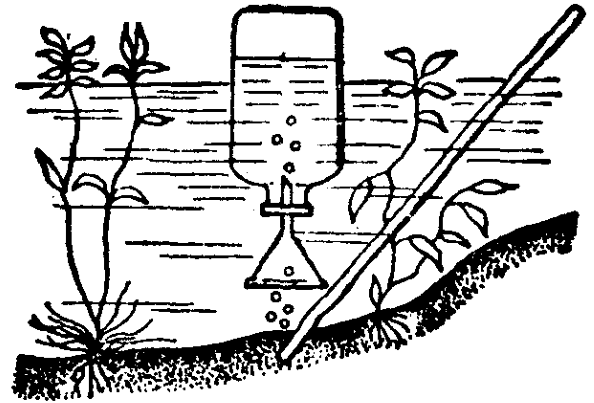
\includegraphics[width=6cm]{../pic/czhx1-ch3-13}
        \caption{在池沼里收集沼气}\label{fig:3-13}
    \end{minipage}
    \qquad
    \begin{minipage}[b]{7cm}
        \centering
        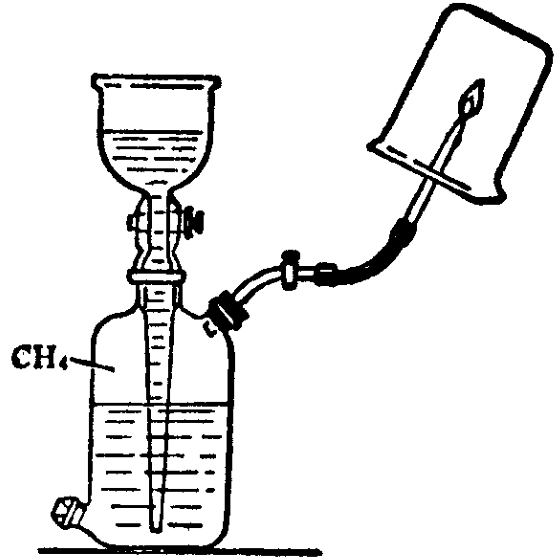
\includegraphics[width=5cm]{../pic/czhx1-ch3-14}
        \caption{甲烷的燃烧}\label{fig:3-14}
    \end{minipage}
\end{figure}

甲烷是一种没有颜色、没有气味的气体。
它比空气轻,极难溶于水,很容易燃烧。

\begin{shiyan}
    点燃从贮气瓶的导管放出的甲烷(点燃前必须象检验氢气纯度那样,先检验甲烷的纯度),观察火焰颜色。
    在火焰上方罩一个冷而干燥的烧杯(图\ref{fig:3-14}),过一会儿,烧杯壁上有什么出现?
    迅速把烧杯倒过来,向杯内注入少量澄清的石灰水,振荡.观察石灰水的变化。
\end{shiyan}

上面的实验说明,甲烷燃烧时生成二氧化碳和水,同时放出大量的热。
\begin{fangchengshi}
    \ce{ CH4 + 2O2 \xlongequal{\text{点燃}} CO2 + 2H2O }
\end{fangchengshi}

点燃甲烷跟氧气或甲烷跟空气的混和物,它就会发生爆炸。
因此在煤矿的矿井里必须采取安全措施(如通风、严禁烟火等),
以防止甲烷跟空气等混和物的爆炸事故发生。

沼气的应用对于解决农村的燃料问题,改善农村环境卫生,提高肥料质量,
以及为实现农业机械化,开辟新的能源以发展农业生产等方面都有重要的意义。

到现在为止,我们已学习过一氧化碳、二氧化碳、碳酸、碳酸钙和甲烷等含碳的化合物,
事实上含碳的化合物很多很多,目前已经知道的已达数百万种,而不含碳的化合物相对来说却少得多。
在含碳的化合物里种类很多,结构也比较复杂,并且有一些共同的性质
(例如,加热时一般容易碳化、容易燃烧, 等等)。
化学上把含碳的化合物叫做有机化合物(简称有机物),
而一般把不含碳的化合物叫做无机化合物,例如水、氯酸钾、氯化锌,等等。
一氧化碳、二氧化碳和碳酸钙等少数物质虽然含有碳元素,
但由于它们的组成和性质跟无机化合物很相似,
因而一向把它们作为无机化合物来研究。
有机化合物跟生物体和工农业生产有密切的关系。

甲烷就是最简单的有机物。乙炔也是一种有机物。
我们日常生活里常常接触到的如酒精、醋酸(食用醋的主要成分)、葡萄糖、
蔗糖、油脂、淀粉、蛋白质、纤维素以及合成纤维、塑料、橡胶等等都是有机物。

由于有机物对国民经济的发展和提高人民生活水平都具有重要的意义,
在近代,生产有机物的各种工业就越来越迅速地发展起来。


\begin{xiti}

\xiaoti{甲烷、氢气和一氧化碳燃烧后,它们的生成物分别是什么,有什么不同,
    能不能以此来鉴别这三种气体?
}

\xiaoti{80 克甲烷充分燃烧,最少需要氧气多少升?最少需要空气多少升(以上气体都在标准状况下)?\\
    (提示:可查阅第一章里的有关数据\footnotemark。)
}
\footnotetext{录注:数据见 第一章 \ref{sec:1-2} \nameref{sec:1-2}}

\end{xiti}


